\chapter{Przyjęta metoda rysowania sceny}
\label{ChapterSceneDrawingMethod}
	Ze względu na założenie uniwersalności - w tym pod względem platformy docelowej - jako podstawa i punkt wyjścia przyjęty został sposób rysowania \textit{Forward Rendering}, ze względu na lepszą skalowalność między systemami o różnej mocy obliczeniowej oraz możliwość użycia większości efektów graficznych. W związku z tym wyborem koszt obliczeniowy oraz pamięciowy rysowania sceny jest bazowo niski, lecz dodanie dużej ilości źródeł światła wiąże się ze zwiększonym narzutem obliczeniowym.
	
\section{Modyfikacja sposobu obliczania oświetlenia}
	Wyraźnym odejściem względem klasycznego \textit{Forward Rendering} jest sposób obliczania oświetlenia. Podstawową metodę można przedstawić w uproszczonej formie przy pomocy pseudokodu w ramach listingu \ref{lst:shaderForwardLightCalculations}.
	
	\begin{lstlisting}[caption={Pseudokod programu cieniującego obliczającego oświetlenie metodą Forward Rendering}, label={lst:shaderForwardLightCalculations}]
UNIFORM Light[] lights; // Przekazane do shader'a dane o źródłach światła,
UNIFORM int numLights;  // oraz o ilości aktywnych źródeł w tablicy.
		
Color resultColor = BLACK;
// Pętla sumująca obliczone wartości oświetlenia
for (i = 0; i < numLights; i += 1) {
    resultColor += CalculateLight(lights[i]);
}

return resultColor; 
	\end{lstlisting}
	
	Takie podejście ma jednak dwa ograniczenia - wydajność oraz ograniczenie maksymalnej ilości źródeł światła w scenie.	Pierwsze wynika ze sposobu działania współczesnych układów graficznych oraz kompilatorów. Dokładniej ograniczenie wydajności wynika z tzw. \textit{Register spilling}, czyli sytuacji w której na układzie graficznym brakuje rejestrów do pełnego pokrycia zmiennych, przez co koniecznym jest korzystanie z powolnej pamięci globalnej \cite{amd:gpuopen:RegisterSpilling}. Możliwym jest też spadek wydajności przez zmniejszenie skuteczności mechanizmu \textit{rozwijania pętli} kompilatora, przez znaczne zwiększenie maksymalnej jej długości. Drugie ograniczenie spowodowane jest limitem ilości elementów bufora stałych w API Direct3D - 4096 \cite{microsoft:Direct3D11:ResourceLimits}, co ogranicza ilość źródeł światła do około 1400. 
	
	Oba problemy zostały rozwiązane dzieląc pełną listę świateł na fragmenty o stałej wielkości (na przykład 64). Następnie zamiast wywoływać proces renderowania dla wszystkich źródeł, uruchamiany jest po kolei dla kolejnych segmentów, a wynik dodawany jest do bufora kolorów przy pomocy mechanizmu \textit{Blending}, opartego o klasę z segmentu \textit{D3DBlendState}. Aby takie podejście działało poprawnie pierwsze wywołanie procesu rysującego odbywa się przy wyłączonym blendingu.
	
	Nowe podejście także może zmniejszać wydajność przy zbyt małej ilości źródeł światła na wywołanie procesu ze względu na konieczność każdorazowego rysowania geometrii i zmiany kontekstów. W związku z tym przeprowadzone zostały testy, z których została określona optymalna wartość świateł na pass - \textbf{64}.
	
	Wizualizacja procesu została pokazana na rys. \ref{Rendering_MultiPassLighting}.
	
		
	\begin{figure}[h!]
		\centering
		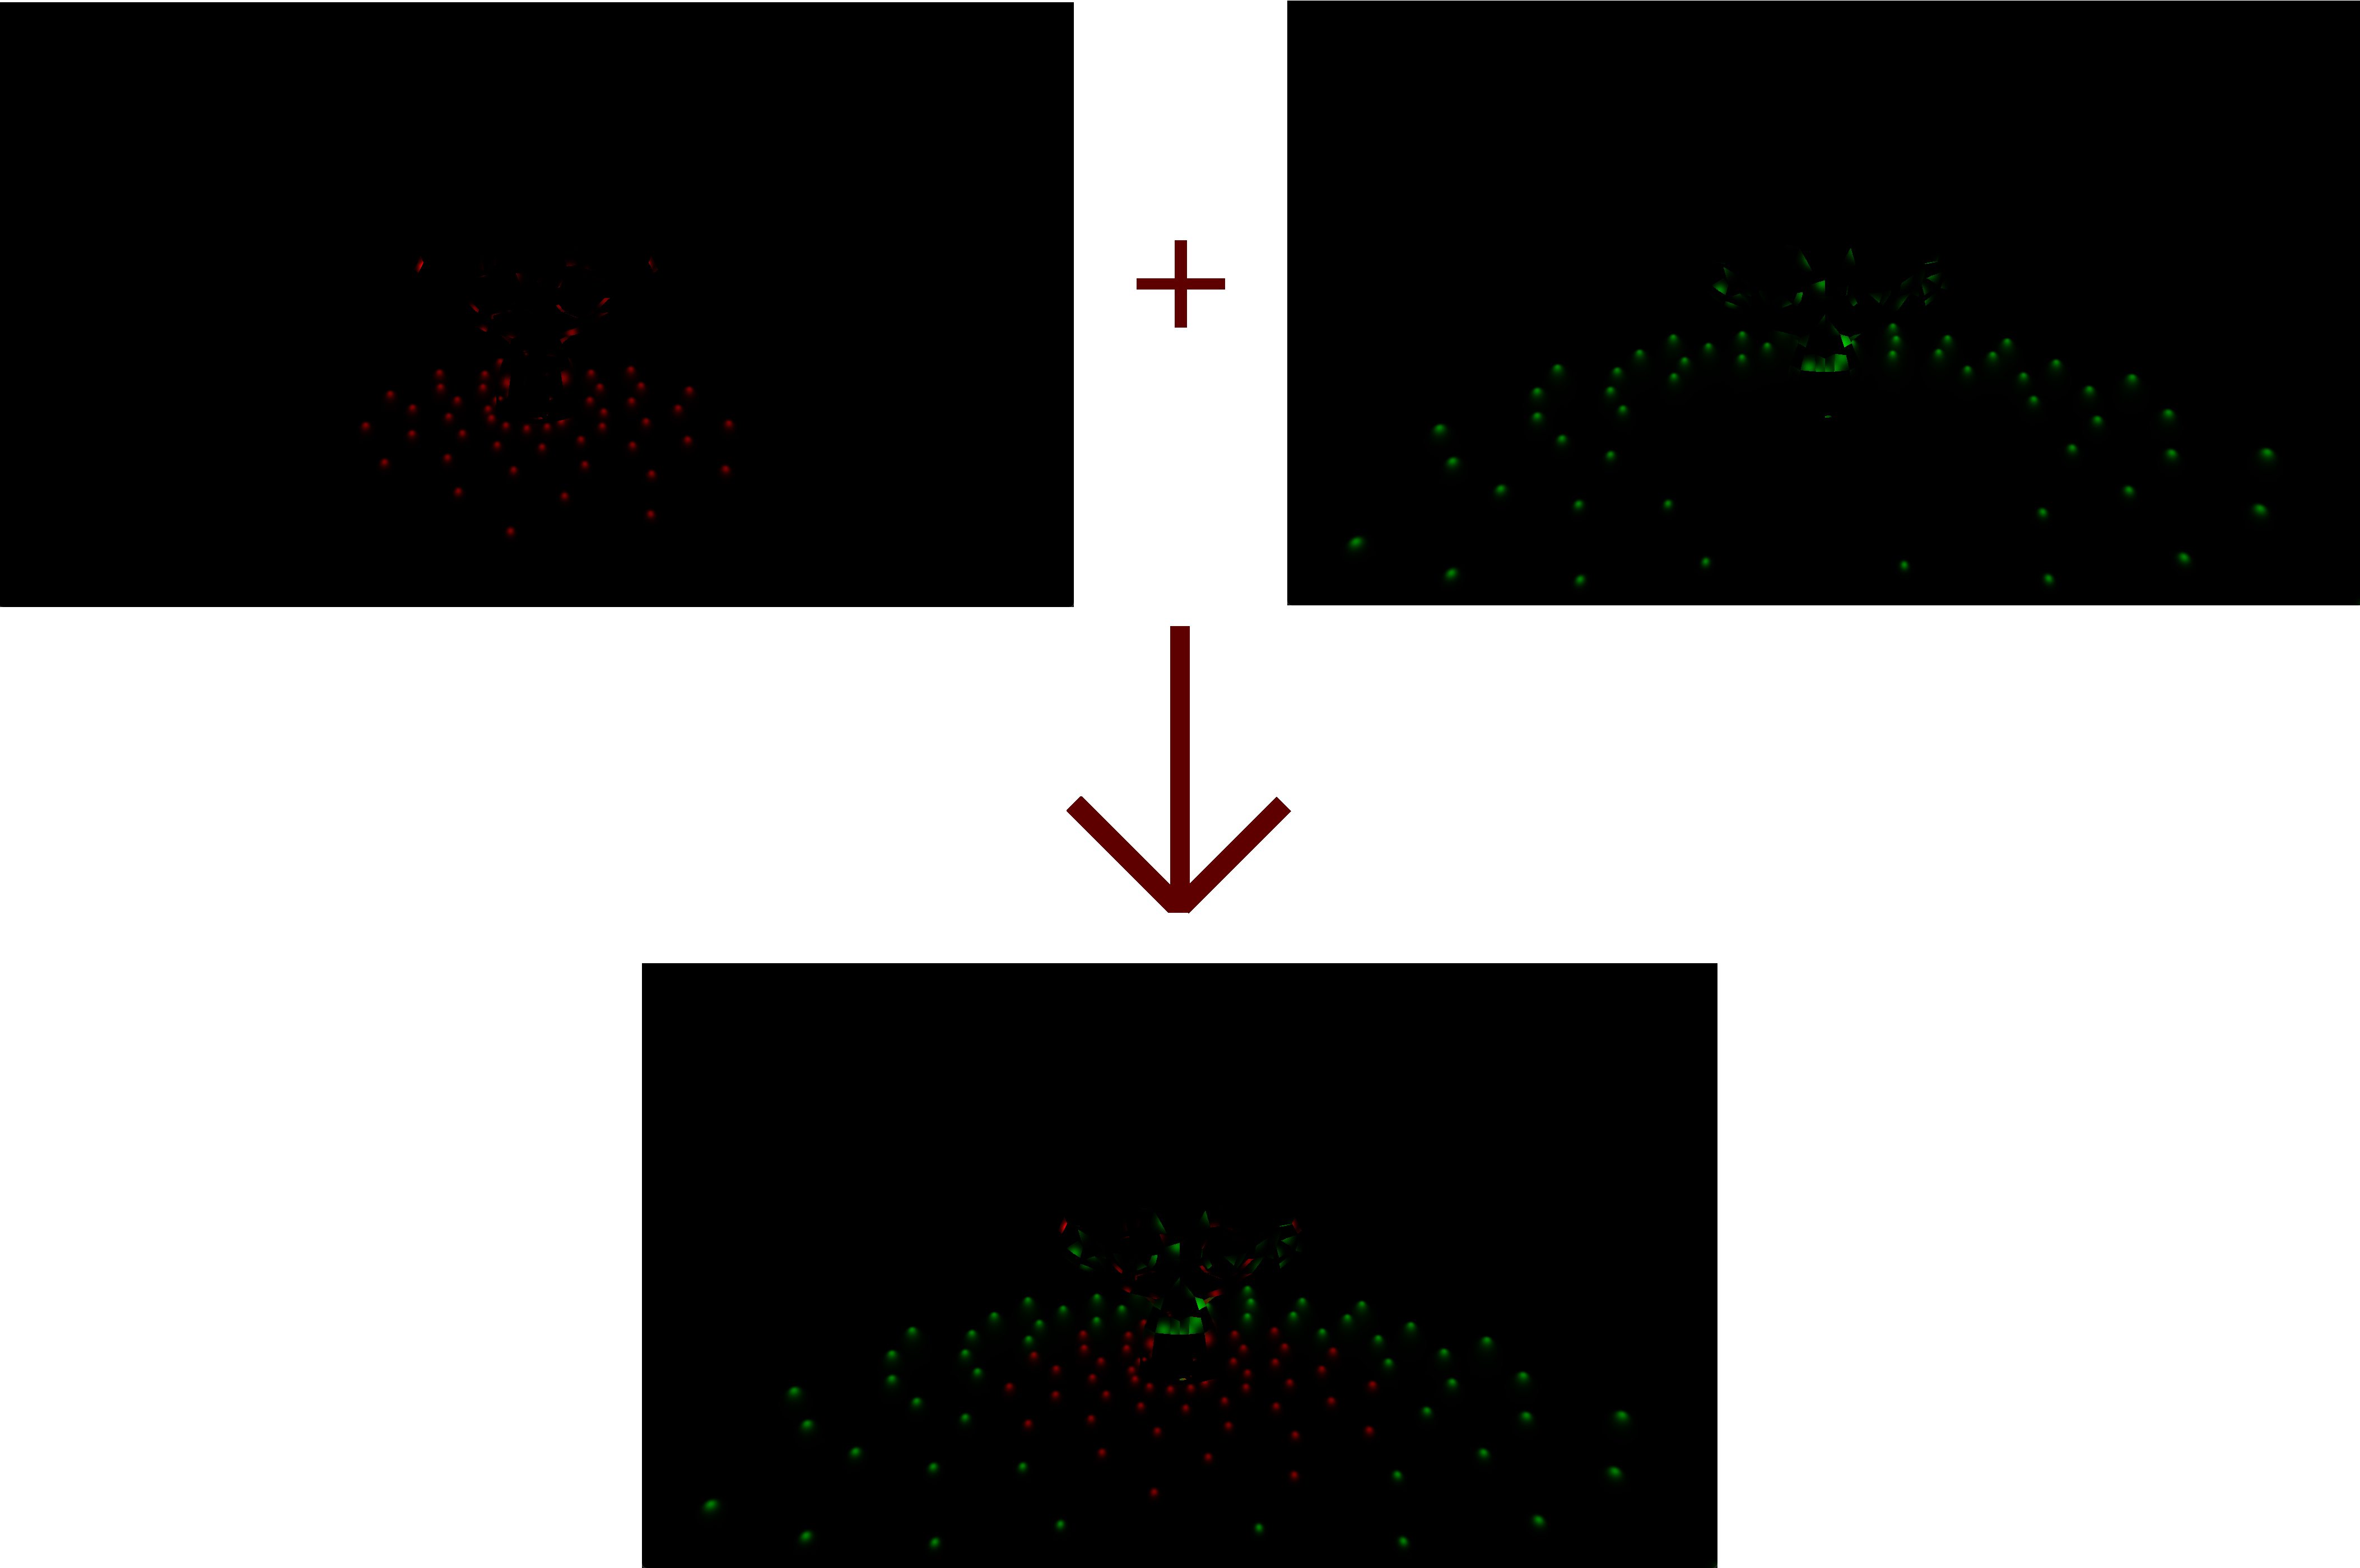
\includegraphics[width=\textwidth]{images/lightsTest_combined.png}
		\caption{Wizualizacja procesu wieloetapowego obliczania oświetlenia.}
		\label{Rendering_MultiPassLighting}
	\end{figure}